\subsection{拓扑向量空间的有界子集}

定义 3. --- 设 E 是一个拓扑向量空间。E 的子集 A 称为有界的，如果它被 E 的每个零邻域吸收（I, 第 7 页, 定义 4）。

要使 A 有界，只需 A 被 0 的某个基本邻域系中的每个邻域吸收。由于存在由 0 的均衡邻域组成的基本邻域系（I, 第 7 页, 命题 4），这等价于说：对 E 中 0 的每个邻域 V，存在 \(\lambda \in K\) ，使得 \(A \subset \lambda V\) 。

假设 E 的拓扑由半范数的一个基本系 \(\Gamma\) 定义（II, 第 3 页）；那么 E 的子集 A 有界，当且仅当每个半范数 \(p \in \Gamma\) 在 A 上有界。

特别地，如果 E 是半赋范空间，E 的子集 A 有界当且仅当它含于某个球中。换言之，如果 E 是赋范的，这就意味着 A 对 E 的度量空间结构是有界的（GT, IX, § 2, No.~2）。

注. --- 1) 如果 E 是半赋范空间，诸球构成 E 中 0 的有界邻域组成的一个基本邻域系。反之，如果 E 是局部凸拓扑向量空间，且 E 中存在 0 的一个有界邻域，则这个邻域包含一个均衡凸邻域 W，而 W 的度规是定义 E 的拓扑的一个半范数。

\pandocbounded{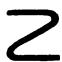
\includegraphics[keepaspectratio]{images/part001_149bf36b.jpg}}

于是，如果 E 是局部凸且可度量化的，且其拓扑不能由单个范数定义，那么 E 上不存在定义其拓扑且使对 \(d\) 而言的有界子集（GT, IX, § 2, No.~2）恰为 E 的有界子集的距离。更确切地说，对 E 上每个平移不变且定义 E 的拓扑的距离 \(d\) ，E 的有界子集对 \(d\) 而言是有界的（III, 第 38 页, 习题 3），但反之不真。

\begin{enumerate}
\def\labelenumi{\arabic{enumi})}
\setcounter{enumi}{1}
\item
  设 M 是 E 的一个向量子空间，赋有诱导拓扑。要使 M 的一个子集在 M 中有界，必须且只需它在 E 中有界。
\item
  设 N 是 E 中 0 的所有邻域之交，于是 \(\tilde{E} = E/N\) 是与 E 相伴的 Hausdorff 向量空间。那么 N 是有界的；如果 \(\pi: E \to \tilde{E}\) 是典范同态，那么 E 的子集 B 有界当且仅当 \(\pi(B)\) 有界。
\item
  设 E 是一个 Hausdorff 局部凸空间；那么对 E 中每个 \(x \neq 0\) ，存在一个连续半范数 p，使得 \(p(x) \neq 0\) ；这个半范数在由 x 生成的实半直线 \(R_{+}.x\) 上不是有界的。因此 E 的任何非零子空间都不是有界的。特别地，有界子集不含任何直线。
\end{enumerate}

定义 4. --- 设 E 是一个局部凸空间。E 上的有界结构 B 称为与 E 适配的，如果它是凸的，由 E 的有界子集组成，且 B 中每个集合的闭包属于 B。

命题 1. --- 设 E 是一个局部凸空间。E 的有界子集所成之集是一个适配有界结构。

我们需要确立下列性质：

\begin{enumerate}
\def\labelenumi{\alph{enumi})}
\item
  如果 \(\mathbf{B}\) 是 \(\mathbf{E}\) 的一个有界子集，那么 \(\mathbf{B}\) 的每个子集都有界。
\item
  两个有界子集的并是有界的。
\item
  与一个有界集位似的每个集合是有界的。
\item
  有界子集的闭均衡凸包（II, 第 13 页）是有界的。
\end{enumerate}

如果 p 是 E 上的一个连续半范数，那么 p 的球是凸的、均衡的、闭的，且与一个球位似的集合还是一个球。因此，如果 p 在 E 的两个子集 X 与 Y 上有界，那么它在 \(X \cup Y\) 的闭均衡凸包上、在与这些集合位似的集合上也都有界。这就确立了性质 b)、c) 与 d)，而 a) 是显然的。

定义 5. --- 设 E 是一个局部凸空间。E 的所有有界子集所成之集称为 E 的典范有界结构。

如果 B 是 E 的有界子集所成的一个集合，那么存在一个与 E 适配且包含 B 的最小有界结构 \(\tilde{B}\) 。\(\tilde{B}\) 中的集合就是那些含于某个集合的集合，该集合与 B 中集合的有限并的闭均衡凸包位似。

每个适配有界结构都含于典范有界结构之中。

命题 2. --- 在局部凸空间 E 中，每个预紧集是有界的。设 A 是 E 的一个预紧子集，V 是 0 的一个均衡凸邻域。存在 A 中点的一个有限序列 \((a_{i})_{1\leqslant i\leqslant n}\) ，使得

\[
\mathrm{A} \subset \bigcup_ {1 \leqslant i \leqslant n} (a _ {i} + \mathrm{V}).
\]

由于 \(B = \{a_{1}, ..., a_{n}\}\) 是有界的，存在一个标量 \(\lambda\) ，使得 \(0 < \lambda < 1\) 且 \(\lambda B \subset V\) ；我们有 \(\lambda A \subset \lambda B + \lambda V \subset V + V\) ，由此命题得证。

推论. --- 在局部凸空间中，一个 Cauchy 序列的点所成之集是有界的。

事实上，这个集合是预紧的（GT, II, § 4, No.~2）。

注 5. --- 一般说来，局部凸空间 E 的有界子集并不都是预紧的（例如，如果 E 是无限维赋范空间，其单位球不是紧的（I, 第 15 页, 定理 3））。然而，当 E 是弱空间（II, 第 42 页）时情形就是如此：因为这时与 E 相伴的 Hausdorff 拓扑向量空间同构于某个乘积 \(K^{I}\) 的子空间，而该乘积的有界子集都是预紧的（参见 III, 第 4 页, 推论 2）。

其他的例子见 IV, 第 18 页。

命题 3. --- 设 A 是局部凸空间 E 的一个子集。假设 A 有界；那么对 A 中点的每个序列 \((x_{n})\) 以及趋于 0 的标量的每个序列 \((\lambda_{n})\) ，序列 \((\lambda_{n}x_{n})\) 趋于 0。反之，如果存在非零标量的一个序列 \((\lambda_{n})\) ，使得对 A 中点的每个序列 \((x_{n})\) ，序列 \((\lambda_{n}x_{n})\) 有界，那么 A 有界。

假设 A 有界。如果 \((\lambda_{n})\) 是趋于 0 的标量序列，且 V 是 0 的一个邻域，那么当 n 充分大时有 \(\lambda_{n}A \subset V\) ，由此第一个断言得证。

反之，如果 A 不是有界的，且 \((\lambda_{n})\) 是一个标量 \(\neq 0\) 的序列，那么存在一个连续半范数 p 与 A 中点的一个序列 \((x_{n})\) ，使得 \(p(x_{n}) \geqslant \frac{n}{|\lambda_{n}|}\) 。于是有 \(p(\lambda_{n}x_{n}) \geqslant n\) ，从而序列 \((\lambda_{n}x_{n})\) 不是有界的。

推论. --- E 的子集 A 有界，当且仅当 A 的每个可数子集有界。

